\section*{Результаты измерений}

\subsection*{Градуировка микрометрического винта}

Проведём калибровку градуировочной шкалы. Цена деления градуировочной шкалы $d_ш = 0,01 \mm$.

\begin{tabular}{|c|c|c|}
	\hline
	№ & 1 & 2 \\
	\hline
	Делений градуировочной шкалы $n_ш$ & 80 & 39 \\
	\hline
	Делений микрометрического винта $n_в$ & 8,19 & 4,00 \\
	\hline
	Цена деления микрометрического винта $d_в$, мкм & $97,7 \pm 0,6$ & $97,5 \pm 1,3$ \\
	\hline
\end{tabular}
$$
d_в = \frac{d_ш \cdot n_ш}{n_в} 
$$

Погрешность определения цены деления микрометрического винта оценивалась по формуле:
$$
\varepsilon_{d_в} = \sqrt{\left(\frac{\sigma_{n_ш}}{n_ш}\right)^2 + \left(\frac{\sigma_{n_в}}{n_в}\right)^2}
$$
где $\sigma_{n_ш} = 0,5$ -- половина деления градуировочной шкалы, $\sigma_{n_в} = 0,005$ -- половина деления микрометрического винта. Измерения производились с помощью микроскопа, поэтому точность результатов определяется, насколько точно человеческий глаз способен определить совпадение делений градуировочной и эталонной шкалы. Для оценки возьмём половину деления, так как система -- механическая, возможен люфт микрометрического винта, деления имеют конечную толщину, а экспериментатор субъективно воспринимает совпадение делений.

За итоговое значение цены деления микрометрического винта возьмём первое измерение, так как у него меньше погрешность измерения: $d_в = 97,7 \pm 0,6 \um$.

\subsection*{Определение радиуса кривизны линзы}

Так как граница между светлым и тёмным кольцом была видна достаточно четко, а середину кольца на глаз определить сложно, то было принято решение измерять координаты границ колец. Координата середины кольца определяется как среднее арифметическое между координатами границ. Для получения радиуса кольца необходимо из координаты середины кольца вычесть координату центра кольца. Измерения проводились в две стороны: влево от центра и вправо от центра, итоговый радиус кольца оценивается как среднее арифметическое между радиусами левых центров колец и правых центров.

Результаты измерений радиусов колец: \\
\begin{tabular}{|c|c|c|c|c|c|c|c|c|c|c|}
	\hline
	№ & 1 & 2 & 3 & 4 & 5 & 6 & 7 & 8 & 9 & 10 \\
	\hline
	$r_{светлые}, \um$ & 85 & 150 & 191 & 227 & 253 & 282 & 305 & 328 & 347 & 367 \\
	\hline
	$r_{тёмные}, \um$ & 123 & 173 & 210 & 240 & 269 & 295 & 318 & 337 & 358 & 376 \\
	\hline
\end{tabular}

Построим график зависимости квадрата радиуса от номера кольца.
\begin{figure}[H]
	\centering
	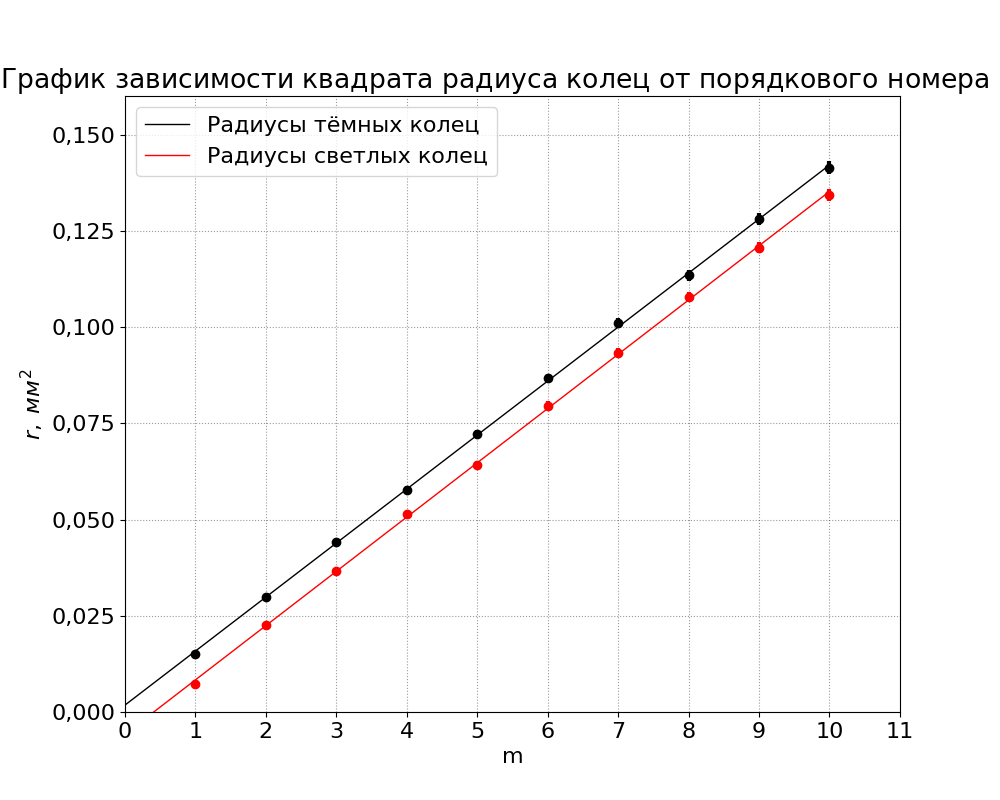
\includegraphics[width=0.6\textwidth]{../Графики/Радиус линзы.png}
\end{figure}

Проведём через экспериментальные точки прямые $y = a x + b$ с помощью метода наименьших квадратов: \\
\begin{tabular}{|c|c|}
	\hline
	$a_с, \mm$ & $0,0141 \pm 0,0001$ \\
	\hline
	$b_с, \mm$ & $-0,0057 \pm 0,0005$ \\
	\hline
	$a_т, \mm$ & $0,0140 \pm 0,0001$ \\
	\hline
	$b_т, \mm$ & $0,0018 \pm 0,0004$ \\
	\hline
\end{tabular}

Длина волны зелёной линии ртути $\lambda = 546,1 \nm$. \\
Оценим радиус кривизны линзы:\\
$R_с = 25,8 \pm 0,1 \mm$. \\
$R_т = 25,7 \pm 0,1 \mm$. \\

Значения радиусов кривизны совпадают в пределах погрешности, поэтому в качестве итогового значения возьмём радиус тёмных колец. \\
$R = 25,8 \pm 0,1 \mm$

\subsection*{Наблюдение биений}

В результате интерференции двух спектральных линий ртутной ламы зелёной $\lambda_2 = 546,1 \nm$ и жёлто-оранжевой $\lambda_1 = 578,2 \nm$ наблюдались биения.

В результате наблюдений было установлено, что количество светлых колец в промежутке между центрами четких систем равно $\Delta m = 17$.

Оценим разность между между спектральными линиями $\Delta \lambda = \frac{\lambda}{\Delta m} = 32,1 \nm$.